\documentclass{article}
    \usepackage{url}
    \usepackage{cite}
    \usepackage{float}   
    \usepackage{xcolor}
    \usepackage{lscape}
    \usepackage{amssymb}
    \usepackage{titling}
    \usepackage{pdfpages}
    \usepackage{enumitem}
    \usepackage{graphicx}
    \usepackage{hyperref}
    \usepackage{fancybox}
    \usepackage{fancyvrb}
    \usepackage{enumerate}
    \usepackage{pdflscape}
    \usepackage{afterpage}
    \usepackage{listings,lstautogobble}    
    \usepackage[margin=0.8in]{geometry}
    \usepackage[nottoc,notlot,notlof]{tocbibind}
    \renewcommand\maketitlehookd{\vfill\null}
    \renewcommand\maketitlehooka{\null\mbox{}\vfill}

    \newcommand\backgroundimage{
        \put(-5,0){
        \parbox[b][\paperheight]{\paperwidth}{
        \vfill
        \centering
        
\includegraphics[height=\paperheight]{Images/background.jpg}
        \vfill
    }}}

    \graphicspath{ {Images/} }

    \title{An Evaluation of Augmented Reality in a Library Using a Microsoft HoloLens
    SENG2260 Assignment 1 \protected{\\}My Dudes
    }
    \author{
        Ethan Bentley
        \texttt{c3130282@uon.edu.au}\\
        Jasbir Shah
        \texttt{c3182837@uon.edu.au}\\
        Jay Rovacsek
        \texttt{c3146220@uon.edu.au}\\
        Josh Brown
        \texttt{c3283797@uon.edu.au}\\
        Dean Morton
        \texttt{c3252227@uon.edu.au}\\
        Tom Milton
        \texttt{c3261280@uon.edu.au}\\
        Ryan Lengling
        \texttt{c3282142@uon.edu.au}\\
        Elijah Hunt
        \texttt{c3236563@uon.edu.au}\\
        Benjamin Walters
        \texttt{c3207457@uon.edu.au}\\
    }

    \date{\today}
    \hypersetup{
    colorlinks=true,
    linkcolor=black,
    filecolor=magenta,      
    urlcolor=blue,
    citecolor=red,
    linktoc=section,
    }
    \pagenumbering{arabic}

    \newlist{legal}{enumerate}{10}
    \setlist[legal]{label*=\arabic*.}

    \begin{document}

    \AddToShipoutPicture{\backgroundimage}

    \begin{titlingpage}
        \maketitle
    \end{titlingpage}

    \tableofcontents
    
    \newpage

    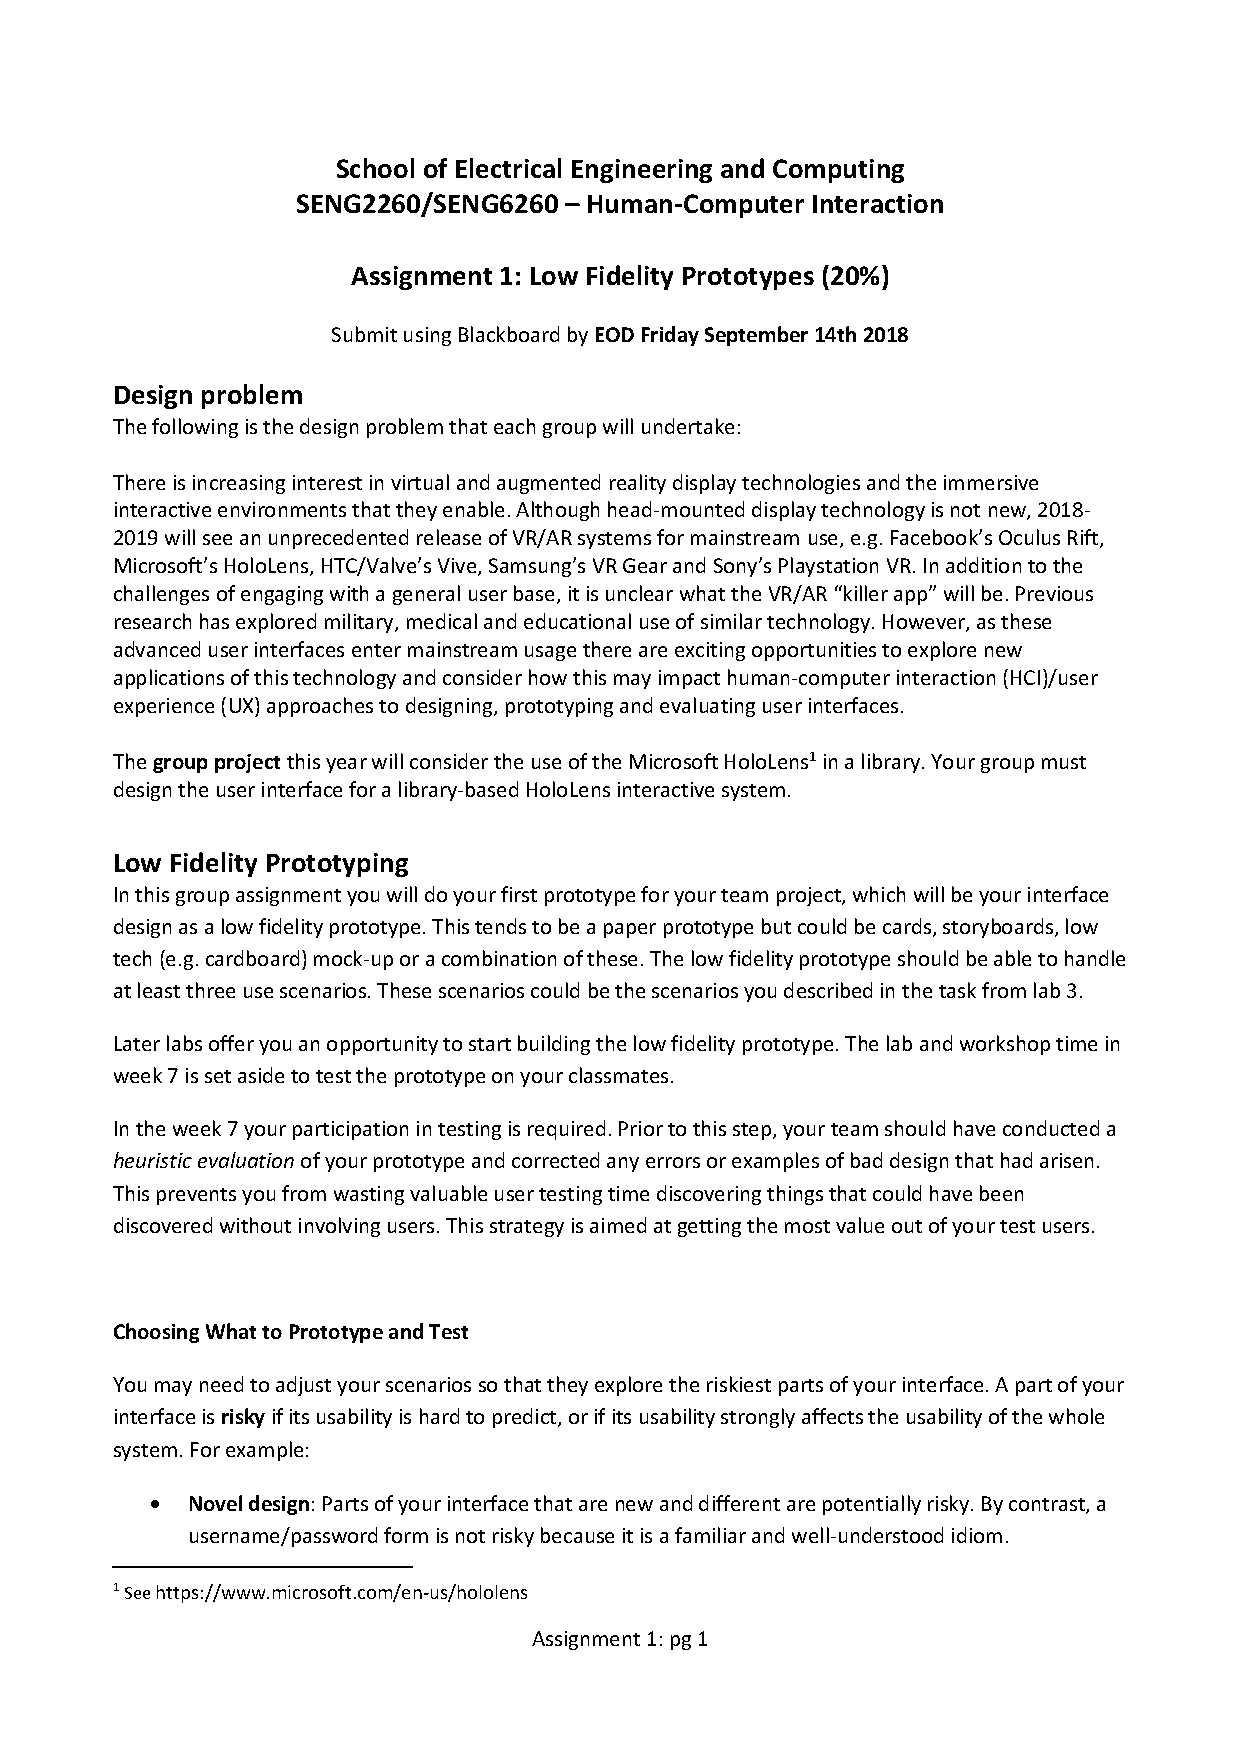
\includepdf[pagecommand=\section{Assignment Requirements},height=\textheight-10pt,keepaspectratio,pages={1}]{Resources/SENG6260_Assignment1_2018.pdf}
    \includepdf[height=\textheight-10pt,keepaspectratio,pages={2}]{Resources/SENG6260_Assignment1_2018.pdf}

    \begin{landscape}
        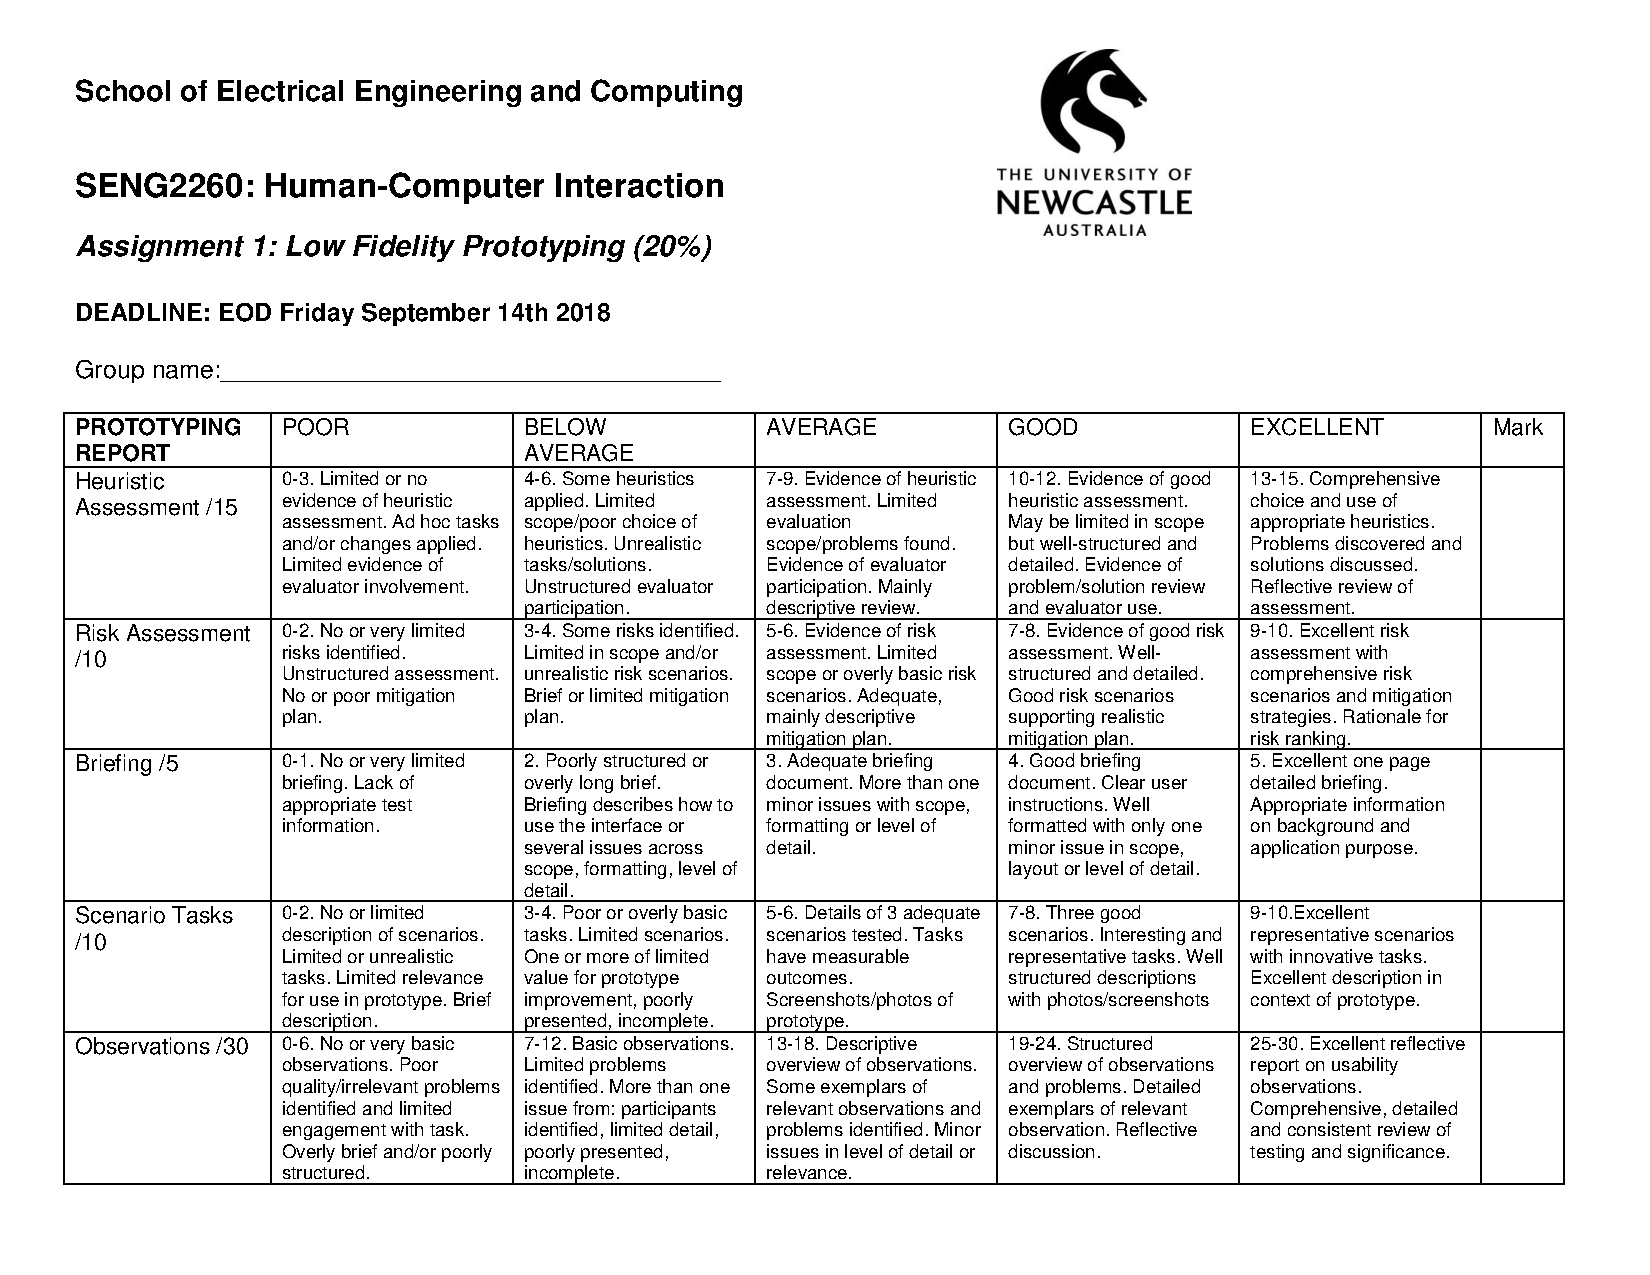
\includegraphics[height=\textheight-10pt,keepaspectratio]{Resources/Marking_Guide.pdf}
        \thispagestyle{empty}
    \end{landscape}
    \newpage

    \section{Project Outline}
    \newpage

    \section{Heuristic Evaluations}
        \subsection{Heuristic Assessment}
            Through the design process we evaluated our user interface using 
            “Jakob Nielsen’s 10 principles for interaction design”. 
            \\
            These heuristics allowed us to make informed decisions when creating 
            and making iterations to our prototype.

            \subsubsection{Visibility of System Status}
                Our prototype gave user feedback by quickly transitioning between 
                slides (screens) based on the user’s gestures. When a user 
                performed a certain gesture it was established that the next 
                slide would be displayed within reasonable time, based on the 
                available performance metrics of the Microsoft Hololens.
                \par
                This type of feedback would allow users to interpret if they had 
                made an error as well as having a ‘screen shake’ effect if the 
                user tried to input a gesture that was not recognised. In the 
                tutorial scenario, if users input a gesture incorrectly then 
                they were given feedback and also shown with an animation of an 
                avatar representing a human hand, how the gesture was to be performed.

            \subsubsection{Match Between System and the Real World}
                The system prototype used a WIMP based metaphor UI display with 
                simple icons and folders to allow users to quickly transition from 
                other computer based systems that use a mouse and keyboard input and 
                mobile based systems which use touch based interfaces - allowing them 
                to quickly adapt to the Hololens gesture input methods.

            \subsubsection{User Control and Freedom}
                The bloom gesture which we associated with the heuristic for ease 
                of use was used as an ‘emergency exit’. If the user became stuck 
                at any point they could use this gesture to return to the main menu. 
                Allowing the user to feel free to explore the menus of the system 
                without the worry of getting lost.

            \subsubsection{Consistency and Standards}
                Consistency was kept in regards to the types of icons displayed 
                and the graphic layout of the icons. This was important as the 
                system transitions between screens frequently and the layout of 
                the icons and menus needs to be logical so as not to confuse the user.
                \par
                The type of error feedback given when a user made an error was also kept 
                consistent in all areas of the system.
            
            \subsubsection{Error Prevention}
                A ‘screen shake’ effect was provided to users as feedback when they attempted 
                to use a gesture incorrectly or when data was input incorrectly. The tutorial 
                scenario was created in an attempt to prevent users from performing gestures 
                incorrectly. This tutorial could be accessed by users at any point if they 
                needed to refresh their memory of what gestures could be performed to perform 
                certain inputs.

            \subsubsection{Recognition Rather Than Recall}
                To decrease the memory load on the user the screens were designed to be 
                minimalist in regards to the amount of information that was displayed per 
                screen. Used in conjunction with the consistency of the icons and layout 
                format of the screens the user was viewing, the user was able to recognize 
                what screen they were on. However, issues presented themselves when the user
                was required to recall what step of the process they were up to.
                \par
                Users frequently checked back to the task checklist while conducting the 
                study, more feedback showing what menu they were currently in and feedback 
                as to what step of the task they were currently on could have helped remedy this.

            \newpage

            \subsubsection{Flexibility and Efficiency of Use}
                Simple hand gestures that the user can quickly learn were used to increase 
                efficiency. This was tested in our Tutorial scenario where we taught new 
                users the commonly used hand gestures to see if they were able to navigate the system. 
                It was decided to keep the amount of gestures low as to not confuse the user.
                When users started becoming familiar with gestures their speed at completing tasks increased.

            \subsubsection{Aesthetic and Minimalist Design}
                The slides which represented different screens being presented to the user only 
                showed relevant information according to which screen was displayed. Allowing the 
                user to easily transition between screens and quickly interpret what information 
                was being displayed. The ‘exit group’ icon was not clear as many users found it hard 
                to find. This could be fixed by making the button larger and separated from the bar.

            \subsubsection{Help Users Recognize, Diagnose and Recover from Errors}
                In the first iteration of the prototype, the error screen contained a webdings 
                type that was to simulate an error message on the error screen. 
                This confused users more as they were not able to recognize that it was an error 
                message and drew the users attention away from the fact that they were being presented 
                with an error screen. This was fixed in future iterations to make the error screen clearer.

            \subsubsection{Help and Documentation}
                The system provides its own tutorial when a new user is recognized. 
                This tutorial is also available at any point from the main menu screen 
                which can be accessed at any time using the bloom gesture.

    \newpage

    \section{Risk Assessment}
    \newpage

    \section{Test User Briefing}
    \newpage

    \section{Team Member Roles}
    \newpage

    \section{Scenario Tasks}
    \newpage

    \section{Observations}
    \subsection{Tutorial Use Case}

    % Please add the following required packages to your document preamble:
    % \usepackage{graphicx}
    \begin{table}[H]
        \begin{tabular}{|l|l|l|l}
        \cline{1-3}
        \multicolumn{3}{|l|}{\textbf{Tester 1}}                                                                                                                                                                                                                                                                                                 &  \\ \cline{1-3}
        \textbf{Tasks}      & \textbf{Observation}                                                                                                                                          & \textbf{Task Duration}                                                                                                                            &  \\ \cline{1-3}
        Open/Close the menu & Was confused, needed help                                                                                                                                     & Overtime                                                                                                                                          &  \\ \cline{1-3}
        Select              & Completed with ease                                                                                                                                           & Reasonable                                                                                                                                        &  \\ \cline{1-3}
        Left/Right          & Did incorrectly twice, needed help                                                                                                                            & Overtime                                                                                                                                          &  \\ \cline{1-3}
        Back/Forward        & Completed with ease                                                                                                                                           & Reasonable                                                                                                                                        &  \\ \cline{1-3}
        Additional Comments & \multicolumn{2}{l|}{Tester Reported Error page was unclear, and wasn’t sure how to proceed. Bloom Gesture was unclear as the tester was not sure if it was simply a gesture or a hand movement. Some text placement was too close to borders. Tester felt more gesture slides would reinforce a better tutorial.} &  \\ \cline{1-3}
        \end{tabular}
        }
        \end{table}

    \newpage

    \section{Risk Resolution and Prototype Iteration}
    \newpage

    \section{Minutes and Summary of Meetings}
    \newpage

    \begin{thebibliography}{9}
        \raggedright
        \bibitem{Placeholder}
            Place \url{holder.com}
    \end{thebibliography}

    \newpage
    \section{Appendix}
    \label{sec:Appendix}
    
    \end{document}